\section{Introduction}

Safe exploration is one of the most studied problems in AI safety \citep{amodei2016concrete}.
The choice between probable safety and the hope of possible discovery presents a dilemma known by many names, from the explore-exploit tradeoff in reinforcement learning to the validity-power tradeoff in statistics.
The optimal balance is problem-dependent, yet general solutions must be problem-independent.
So, to apply to real-world problems, any general solution must encode this balance as a hyperparameter, which then must be tuned from data or derived from assumptions about problem structure.
In consequential settings, collecting data from an unsafe behavior policy (a context-dependent strategy or distribution over actions) may be unacceptable. 
Deriving the balance from assumptions about the problem reintroduces a subtler form of
problem-dependence, namely the practitioner's understanding of the setting itself.
% the following sentence structure mirrors the preceding two sentences
Yet consequential, poorly understood settings are precisely where machine learning offers the greatest potential benefit.

\begin{figure*}
    \centering
    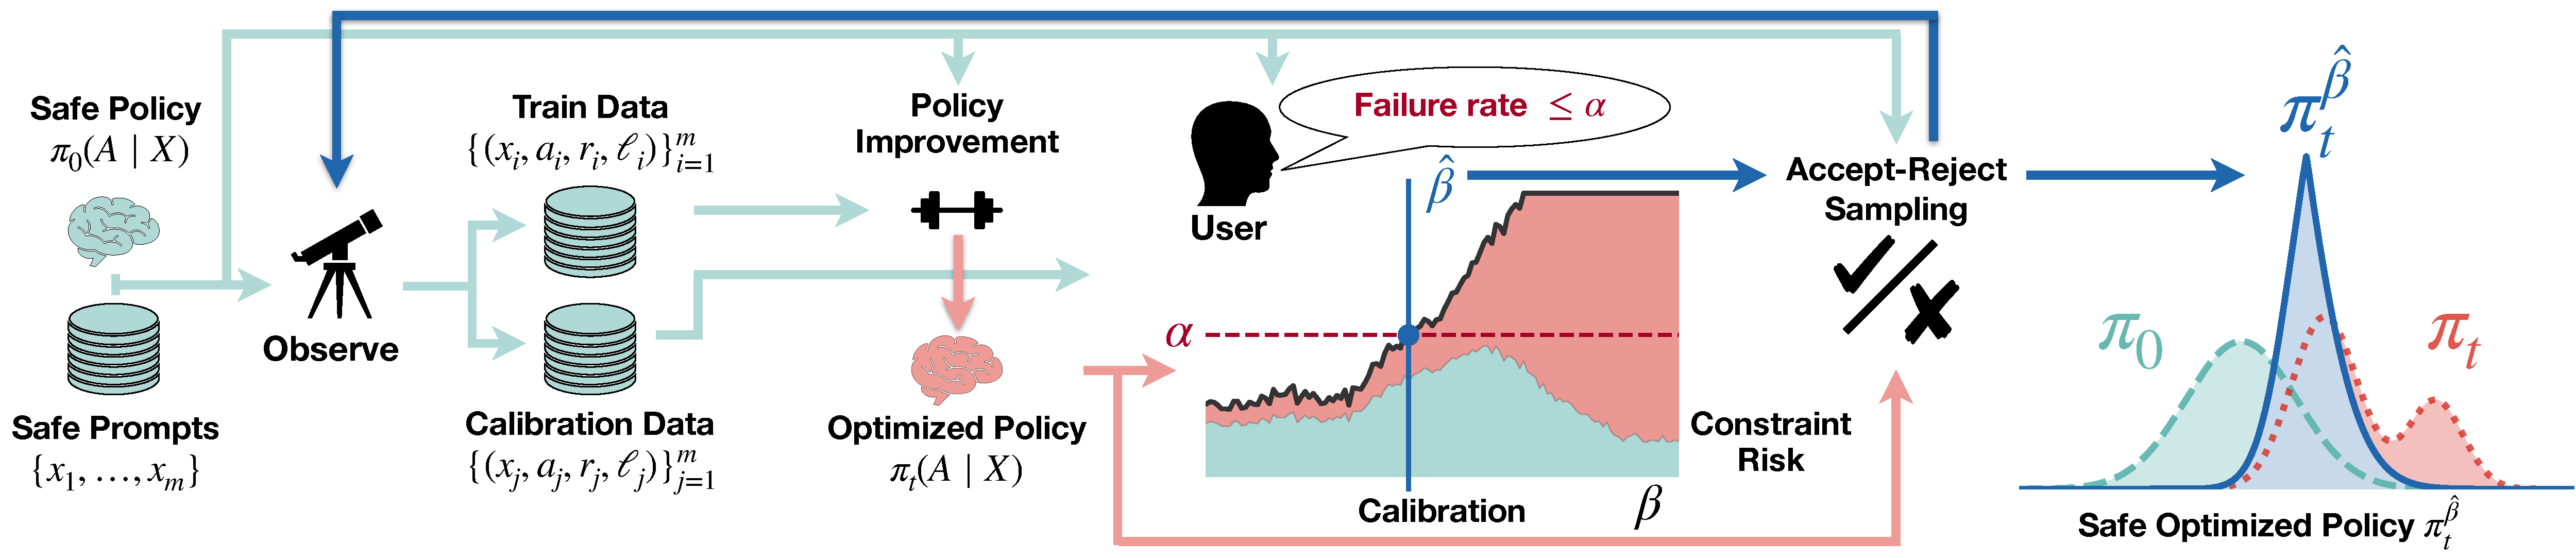
\includegraphics[width=\linewidth]{figures/safe_policy_improvement_fig_1.pdf}
    \caption{
        An illustration of safe exploration with conformal policy control.
        Starting with a safe policy $\pi_0$  and safe context prompts $\mathcal{X}_0:=\{x_1, \dots, x_m\}$, we observe the safe policy's actions $a_i$ and corresponding reward $r_i \in \mathbb{R}$ and constraint violation $\ell_i \in \{0, 1\}$.
        We split the observations into train and calibration data, and optimize the safe policy to obtain $\pi_t$. We then query the user for their constraint violation risk tolerance $\alpha$, and apply conformal risk control to find a bound on the likelihood ratio $\pi_t / \pi_0$ which guarantees the calibrated risk is controlled at level $\alpha$.
        Finally we apply rejection sampling to probabilistically regulate the optimized policy for deployment and observation, allowing the user to flexibly trade off reward, constraint risk, and test-time compute.
    }
    \label{fig:safe_policy_improvement_marquee}
\end{figure*}

Consider an agent that observes contexts (i.e., states) and takes actions to maximize reward while satisfying safe operating constraints to within some tolerance.
  For example, a language model responding to medical questions aims to give answers that are as helpful as possible while avoiding false claims.
  In biomolecular engineering, a generative model proposing improvements to lead molecules aims to maximize efficacy of its designs while ensuring that they are synthesizable.
In such settings, the agent has candidate policies optimized for performance but does not yet know which, if any, are safe to deploy.
  From past experience, the agent usually has a default safe policy it knows controls the risk, but playing it safe may be far from optimal.
  
  What the safe policy does supply is calibration data: Reweighting each observation by a candidate-to-safe likelihood ratio gives an estimate of each candidate's risk.
  % When that ratio is bounded, a weighted estimate suffices to evaluate whether to expect that a candidate's risk exceeds the declared tolerance.
  But which candidate should the agent deploy?
  The natural move is to estimate every candidate's risk and pick the most aggressively optimized one that still looks safe, but this approach introduces bias: Selection corrupts the procedure by favoring estimates that understate their true risk.
  % , so the act of choosing corrupts the estimate that justified the choice.
  Yet the change in risk the agent must control is due to the policy shift it will author.
  The agent does not know how the world will respond to a given action, but it knows exactly how each candidate would distribute its actions, which is the only difference between the distributions it has experienced in the past and those it would encounter in the future.\footnote{If we assume the environment is stationary.}
  %and that is the only difference between the distributions of the data it has and the data it would face.
  
% Consider an agent that observes contexts (i.e. states) and takes actions to maximize reward while satisfying safe operating constraints.
% For example, a language model responding to medical questions aims to give answers that are as helpful as possible while avoiding false claims.
% In biomolecular engineering, a generative model proposing improvements to lead molecules aims to maximize efficacy of its designs while ensuring that they are synthesizable. 
% In such settings, the agent tunes an optimized policy for future performance but does not yet know if it is safe.
% From past experience, the agent usually has a default safe policy it knows controls the risk, but playing it safe may be far from optimal. 
% The agent can reweight the safe policy's data to estimate the risk of a candidate policy, and if the likelihood ratio between the two policies is bounded, these importance weights are bounded, and the safe policy's data suffices to determine whether the candidate's risk exceeds the declared tolerance.
% But which candidate should the agent deploy? The natural move (estimate every candidate's risk, deploy the most aggressive one that looks safe) is biased: among many uncertain estimates, selection favors whichever most understates its true risk, so the act of choosing corrupts the estimate that justified the choice. Yet the shift the agent must correct for is one it authored. The agent does not know how the world will respond to any given action, but it knows exactly how each candidate would distribute its actions, and that is the only difference between the data it has and the data it would face.
% But which candidate should the agent deploy? The weights depend on the deployed policy, and the deployed policy depends on the weighted risk estimates.
% How should the agent proceed? Rather than assuming knowledge of the problem, we resolve this circularity by exploiting what the agent knows about itself.

We introduce conformal policy control (CPC, Figure~\ref{fig:safe_policy_improvement_marquee}), a method for safe exploration that uses the calibration data to interpolate between any safe and any optimized policy while provably respecting the risk tolerance. 
CPC requires no assumptions on the reward or constraint functions, no access to the optimized policy's training process, and no additional samples to tune the balance beyond what a safe policy already provides.
The key idea is to invert the usual importance-weighting paradigm: Rather than estimating risk for a fixed policy, we search over candidate policies, parameterized by a likelihood-ratio threshold, for the most aggressive one such that all evaluated candidates still satisfy the risk tolerance (with a weighted conservative adjustment). Conformal calibration on the safe policy's data determines both the weights and the threshold.
At deployment, the interpolated policy can be realized through rejection sampling (or other Monte Carlo methods), which allows the agent to probabilistically self-regulate to a zone of competence determined by its calibration data.
Because CPC operates entirely at test time, the same safe and optimized policies can be reused under different risk tolerances, trading test-time compute for risk control without retraining.

Providing finite-sample guarantees in this setting poses several challenges for uncertainty quantification. The deployed policy depends on the calibration data, introducing subtle, data-dependent distribution shift. 
The relevant losses are general constraint functions, not just coverage indicators. 
Conformal risk control (CRC) \citep{angelopoulos2022conformal} can address these challenges, but assumes a monotone relationship between the control parameter and the loss. In CPC, the loss function does not depend on the control parameter, so the monotonicity assumption does not hold. We generalize CRC (gCRC) to non-monotonic bounded loss functions, and we prove that CPC inherits finite-sample guarantees when the control parameter governs the policy, not the loss.
% While gCRC requires Lipschitz continuity of the loss in the control parameter, CPC's control parameter acts on the likelihood ratio rather than the loss. The regularity condition thus falls on the policy, which the agent knows and controls, rather than on the constraint function, which it does not.

% We validate our method on three tasks. In medical question answering, we control the false discovery rate, a non-monotonic loss that standard CRC cannot handle directly. In constrained active learning, the agent's actions induce feedback-loop shifts that violate standard exchangeability assumptions. In black-box sequence optimization, a language model agent must improve biomolecular sequences while respecting a constraint budget.
% In each setting, CPC provides finite-sample risk control from the first round of deployment, without hyperparameter tuning or structural assumptions. In medical question answering, this yields tighter risk control and better claim recall than existing methods. In active learning, we obtain finite-sample guarantees where previous approaches provide only asymptotic control. In sequence optimization, we extend conformal methods to a setting where no prior guarantees existed, and find that moderate risk control can counterintuitively improve optimization performance by stabilizing the algorithm. Safe exploration is not only safe, it can also be more efficient.

We validate our methods on three tasks. In medical question answering, gCRC controls the false discovery rate, a non-monotonic loss that standard CRC cannot
  handle, achieving tighter control and better claim recall than existing methods. In constrained active learning, CPC provides finite-sample guarantees under
  feedback-loop covariate shifts where previous approaches offered only asymptotic control. In black-box biomolecular sequence optimization, CPC extends conformal
  methods to a setting where no prior guarantees existed, and we find that moderate risk control can counterintuitively improve optimization performance by reducing
   wasted evaluations on infeasible actions. Safe exploration is not only safe, it can also be more efficient.
